\documentclass[tikz, border=10pt]{standalone}
\usepackage{tikz}
\usetikzlibrary{shapes, positioning, arrows.meta, calc, backgrounds}

\begin{document}
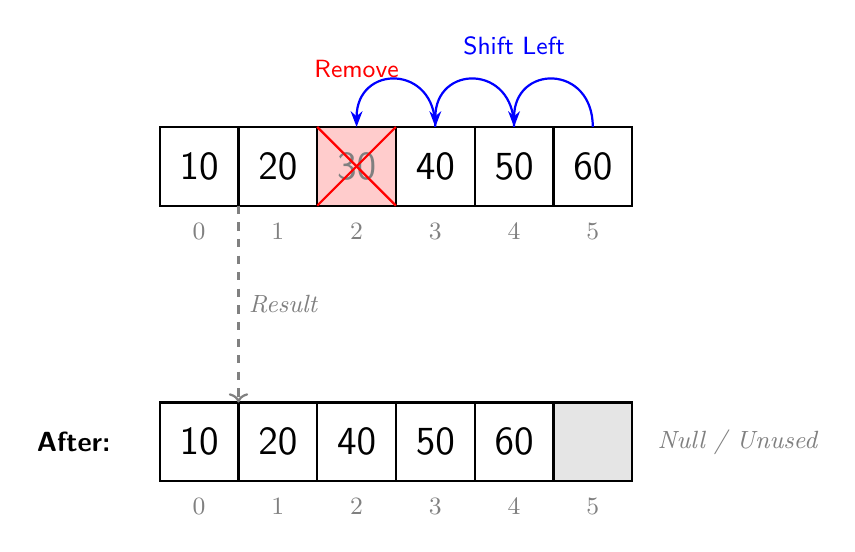
\begin{tikzpicture}[
    cell/.style={
        rectangle, 
        draw=black, 
        thick, 
        minimum width=1cm, 
        minimum height=1cm, 
        node distance=0cm, 
        outer sep=0pt,
        font=\Large\sffamily
    },
    index/.style={
        font=\small\ttfamily\color{gray},
        below=0.1cm of #1
    },
    arrow/.style={
        ->, 
        thick, 
        color=blue, 
        >={Stealth[length=2mm]}
    },
    removed/.style={
        fill=red!20,
        text=gray
    }
]

    % -- Initial State --
    \node[cell] (c0) {10};
    \node[cell, right=of c0] (c1) {20};
    \node[cell, right=of c1, removed] (c2) {30}; % Element to remove
    \node[cell, right=of c2] (c3) {40};
    \node[cell, right=of c3] (c4) {50};
    \node[cell, right=of c4] (c5) {60};

    % Indices
    \node[below=0.1cm of c0, font=\small\color{gray}] {0};
    \node[below=0.1cm of c1, font=\small\color{gray}] {1};
    \node[below=0.1cm of c2, font=\small\color{gray}] {2};
    \node[below=0.1cm of c3, font=\small\color{gray}] {3};
    \node[below=0.1cm of c4, font=\small\color{gray}] {4};
    \node[below=0.1cm of c5, font=\small\color{gray}] {5};

    % Cross out removed element
    \draw[red, thick] (c2.north west) -- (c2.south east);
    \draw[red, thick] (c2.north east) -- (c2.south west);
    \node[above=0.5cm of c2, font=\small\sffamily\color{red}] {Remove};

    % Arrows showing left shifts
    % Shift 40 to 2
    \draw[arrow] (c3.north) .. controls +(up:0.8cm) and +(up:0.8cm) .. (c2.north);
    % Shift 50 to 3
    \draw[arrow] (c4.north) .. controls +(up:0.8cm) and +(up:0.8cm) .. (c3.north);
    % Shift 60 to 4
    \draw[arrow] (c5.north) .. controls +(up:0.8cm) and +(up:0.8cm) .. (c4.north);

    % Label for shift operation
    \node[above=0.8cm of c4, font=\small\sffamily\color{blue}] {Shift Left};


    % -- Final State --
    \node[below=2.5cm of c0, cell] (f0) {10};
    \node[below=0.1cm of f0, font=\small\color{gray}] {0};

    \node[cell, right=of f0] (f1) {20};
    \node[below=0.1cm of f1, font=\small\color{gray}] {1};

    \node[cell, right=of f1] (f2) {40};
    \node[below=0.1cm of f2, font=\small\color{gray}] {2};

    \node[cell, right=of f2] (f3) {50};
    \node[below=0.1cm of f3, font=\small\color{gray}] {3};

    \node[cell, right=of f3] (f4) {60};
    \node[below=0.1cm of f4, font=\small\color{gray}] {4};

    \node[cell, right=of f4, fill=gray!20] (f5) {}; % Empty/Null
    \node[below=0.1cm of f5, font=\small\color{gray}] {5};

    \node[left=0.5cm of f0, font=\sffamily\bfseries] {After:};
    \node[right=0.2cm of f5, font=\small\itshape\color{gray}] {Null / Unused};

    % Arrow connecting states
    \draw[transform canvas={xshift=-2cm}, ->, thick, gray, dashed] ($(c0.south west)!0.5!(c5.south east)$) -- node[midway, right, font=\small\itshape] {Result} ($(f0.north west)!0.5!(f5.north east)$);

\end{tikzpicture}
\end{document}
